\documentclass{technology_watch}

\usepackage[french]{babel}
\frenchsetup{SmallCapsFigTabCaptions=false}
\usepackage{siunitx}
\sisetup{locale=FR,retain-explicit-plus=true}
\usepackage{placeins}
\usepackage{flafter}
\captionsetup{hypcap=false}
\setlength{\textfloatsep}{10pt plus 2pt minus 2pt}
\setlength{\dbltextfloatsep}{10pt plus 2pt minus 2pt}
\clubpenalty=10000
\widowpenalty=10000
\displaywidowpenalty=10000
\brokenpenalty=10000
\newcommand{\CorpusRecordings}{3591}
\newcommand{\CorpusSupported}{3492}
\newcommand{\CorpusSpecies}{296}
\newcommand{\NoiseRecordings}{2937}
\newcommand{\CorpusFailed}{108}
\newcommand{\CorpusUndetected}{555}
\newcommand{\CorpusUnsupported}{99}
\newcommand{\CorpusCountries}{96}
\newcommand{\OverlapPairs}{1416}
\newcommand{\CorpusHours}{51.2}
\newcommand{\SpeciesSingleton}{148}

\newcommand{\NBPTwoThreshold}{0.05}
\newcommand{\NBPTwoFOne}{0.425}
\newcommand{\NBPThreeThreshold}{0.05}
\newcommand{\NBPThreeFOne}{0.664}
\newcommand{\HSNTwoThreshold}{0.50}
\newcommand{\HSNTwoFOne}{0.655}
\newcommand{\HSNThreeThreshold}{0.05}
\newcommand{\HSNThreeFOne}{0.603}
\newcommand{\NBPCalibratedDifference}{+0.239}
\newcommand{\NBPCalibratedLower}{+0.200}
\newcommand{\NBPCalibratedUpper}{+0.278}
\newcommand{\HSNCalibratedDifference}{-0.052}
\newcommand{\HSNCalibratedLower}{-0.123}
\newcommand{\HSNCalibratedUpper}{+0.016}
\newcommand{\NBPControlledClean}{75.5}
\newcommand{\NBPGaussianZero}{63.8}
\newcommand{\NBPNaturalZero}{70.2}
\newcommand{\HSNControlledClean}{45.0}
\newcommand{\HSNGaussianZero}{22.2}
\newcommand{\HSNNaturalZero}{29.2}
\newcommand{\NBPControlledPairs}{20}
\newcommand{\NBPIsolatedBoth}{60.0}
\newcommand{\NBPMixedBoth}{30.0}
\newcommand{\HSNControlledPairs}{19}
\newcommand{\HSNIsolatedBoth}{26.3}
\newcommand{\HSNMixedBoth}{5.3}


\VeilleTitle{Reconnaissance acoustique des oiseaux par apprentissage profond}
\VeilleShortTitle{Bioacoustique : robustesse et généralisation}
\VeilleSubtitle{Rapport final de veille technologique}
\VeilleAuthor{Maxime DRÉAN}
\VeilleDate{Octobre 2026}
\VeilleCourse{Master 2 -- Outils Méthodologiques pour la Recherche et l'Entreprise -- Informatique 2349}
\renewcommand{\watchauthorlabel}{Nom -- Prénom :}
\renewcommand{\watchdatelabel}{Date :}
\renewcommand{\watchabstractlabel}{Résumé --}
\renewcommand{\watchkeywordslabel}{Mots-clés --}
\renewcommand{\watchquestionlabel}{Question de veille --}
\addto\captionsfrench{\renewcommand{\refname}{Références}\renewcommand{\tablename}{Tableau}}

\newcommand{\ReportDataset}{Jeu}
\newcommand{\ReportVersion}{Version}
\newcommand{\ReportThreshold}{Seuil}
\newcommand{\ReportSourceSplit}{\shortstack{Sources\\calibration / test}}
\newcommand{\ReportPrecision}{Précision}
\newcommand{\ReportRecall}{Rappel}
\newcommand{\ReportFOneNineFiveInterval}{F1 micro [IC 95\,\%]}

\begin{document}
\raggedbottom

\MakeVeilleTitle
{Cette veille compare la reconnaissance directe et le transfert de
représentations pour identifier les oiseaux dans des enregistrements naturels.
Les publications et les outils disponibles font apparaître trois difficultés :
le masquage acoustique, les annotations incomplètes et le changement de domaine.
Une expérimentation sur BirdNET 2.4 et 3.0 confronte ces difficultés à des
segments annotés et à des perturbations contrôlées. Elle montre une dégradation
sous bruit et superposition, ainsi qu'une comparaison des versions sensible au
jeu et au seuil. Le choix d'un outil demande donc une validation adaptée au
terrain ; la seule architecture ou l'étendue du vocabulaire ne le détermine pas.}
{bioacoustique ; BirdNET ; transfert d'apprentissage ; bruit ; polyphonie ; généralisation.}
{Dans quelle mesure les modèles d'apprentissage profond permettent-ils de
détecter et d'identifier automatiquement les espèces d'oiseaux à partir
d'enregistrements réalisés en milieu naturel, malgré le bruit ambiant, les
vocalisations simultanées et la variabilité géographique ?}

\section{Question de veille et périmètre}

Le suivi acoustique passif fournit des enregistrements répétés sans observation
continue sur le terrain. Leur analyse manuelle limite le volume exploitable.
L'apprentissage profond automatise une partie de l'identification, mais une
liste d'espèces prédites doit encore être confrontée aux vocalisations présentes
pour servir un suivi écologique\cite{stowell2022,kahl2021}.

La question initiale associait le bruit, les vocalisations simultanées et la
variabilité géographique. Ces trois axes sont conservés dans la veille. Le
volet expérimental s'est précisé : l'exploration de sons Xeno-canto a été
complétée par une comparaison sur des paysages sonores annotés, puis par des
perturbations avec témoins. Cette évolution répond à la difficulté d'interpréter
un score sans référence suffisante. L'étude porte sur les chants et les cris,
sans localisation spatiale, estimation d'abondance ou mesure des limites
temporelles des vocalisations. La géographie reste une question documentaire,
faute d'un test isolant son effet de celui des espèces et des conditions de
collecte.

La sélection part de Stowell, de BirdNET et de BirdSet, puis examine le transfert,
l'auto-supervision et les évaluations de terrain. Les critères de comparaison
sont les données et objectifs d'apprentissage, les sorties, l'adaptation,
l'évaluation et le déploiement. Les articles étayent les résultats ; les dépôts
et fiches de modèles documentent les versions, formats et licences. Les travaux
sont retenus pour éclairer ces critères, sans viser une revue systématique.

Trois questions guident la comparaison : le modèle couvre-t-il les catégories
recherchées, ses représentations peuvent-elles être adaptées, et les conditions
d'évaluation correspondent-elles à l'usage envisagé ? Cette distinction évite
de confondre un gain sur un jeu de référence avec une amélioration directement
transférable au suivi d'un site.

\section{Approches disponibles et verrous technologiques}

\subsection{Reconnaissance directe ou représentations à adapter}

BirdNET associe des spectrogrammes à un vocabulaire appris d'espèces
\cite{kahl2021}. Sa version 2.4 repose sur un réseau de type EfficientNet-B0 ;
la documentation des fichiers distribués complète la description du système
initial\cite{birdnetmodels,birdnet24weights}. Perch 2.0 conserve une supervision
sur des corpus annotés de plusieurs taxons, avec un EfficientNet-B3. Il produit
des scores et des représentations sur des segments de cinq secondes à 32~kHz
\cite{perch2025}. La reconnaissance directe évite un entraînement local, tant que
les catégories recherchées sont couvertes. Le transfert réutilise au contraire
l'encodeur pour apprendre une décision adaptée aux données ou catégories locales.
Le tableau~\ref{tab:technologies} résume les usages et adaptations possibles.

\begin{table*}[!t]
\centering\small
\caption{Comparaison des solutions retenues dans la veille. Seul BirdNET est
exécuté dans l'expérimentation ; les autres lignes synthétisent les sources citées.}
\label{tab:technologies}
\begin{tabularx}{\textwidth}{@{}>{\raggedright\arraybackslash}p{1.8cm}YYY@{}}
\toprule
Modèle & Apprentissage et signal & Sorties et adaptation & Conséquence pour le choix \\
\midrule
BirdNET\newline\cite{kahl2021,birdnetmodels} & Supervision ; spectrogrammes ;
réseau de type EfficientNet-B0 pour 2.4 & Scores d'espèces, représentations
et classifieur personnalisé & Analyse directe si le vocabulaire couvre
la cible ; seuil à vérifier sur les données locales \\
Perch 2.0\newline\cite{perch2025} & EfficientNet-B3 ; corpus annotés de
plusieurs taxons & Scores et représentations pour transfert & Même encodeur
pour reconnaissance directe et adaptation à des catégories locales \\
AVES\newline\cite{aves2023} & HuBERT ; forme d'onde ; prédiction d'unités
masquées & Représentations audio à adapter & Choisir la configuration de
préentraînement et entraîner une décision pour la tâche visée \\
Bird-MAE\newline\cite{birdmae2025} & ViT ; spectrogrammes ; reconstruction
masquée sur BirdSet-XCL & Ajustement du réseau ou classifieur sur
représentations gelées & Comparer aussi les têtes linéaires et à prototypes
avec les mêmes annotations \\
\bottomrule
\end{tabularx}
\end{table*}

Perch 2.0 combine notamment Xeno-canto, iNaturalist, Tierstimmenarchiv et
FSD50K. Son apprentissage associe une auto-distillation entre têtes de
classification à la prédiction de l'enregistrement source\cite{perch2025}.
La supervision ne se réduit donc pas au nom d'espèce. Ses deux sorties
permettent d'essayer la classification distribuée, puis de réutiliser
l'encodeur si les catégories locales demandent une adaptation.

Ghani et al. montrent en 2023 que des représentations aviaires issues notamment
de BirdNET et de Perch servent efficacement plusieurs tâches bioacoustiques
avec un classifieur linéaire\cite{ghani2023}. Leur étude de 2025 précise le
compromis : la distillation est favorable sur les données Xeno-canto du domaine
étudié, tandis qu'une adaptation limitée du classifieur associé à BirdNET
généralise mieux aux paysages sonores évalués\cite{ghani2025}. Ajuster davantage
de paramètres n'assure donc pas un meilleur transfert. Le choix porte aussi sur
les données d'adaptation et sur les paramètres conservés.

AVES et Bird-MAE réduisent la dépendance aux annotations pendant le
préentraînement, mais construisent des tâches différentes. AVES applique une
approche HuBERT à la forme d'onde et prédit des unités acoustiques masquées, à
partir de combinaisons de FSD50K, AudioSet et VGGSound\cite{aves2023}.
Bird-MAE emploie un Vision Transformer (ViT) pour reconstruire des portions
masquées de spectrogrammes, sur le sous-ensemble aviaire XCL de BirdSet
\cite{birdmae2025}. Le premier vise des représentations audio généralistes ou
bioacoustiques ; le second spécialise son préentraînement sur les oiseaux.

Les représentations doivent aussi être associées à une décision. Bird-MAE
étudie des têtes à prototypes qui exploitent mieux ses caractéristiques gelées
qu'une simple tête linéaire dans les expériences publiées\cite{birdmae2025}.
Les performances dépendent ainsi de l'encodeur, du classifieur et du protocole.
Les différences de données empêchent d'attribuer les écarts publiés à la seule
opposition entre réseaux convolutifs et Transformers. L'auto-supervision
économise des annotations de préentraînement, mais l'adaptation et l'évaluation
en demandent encore.

\subsection{Annotations, masquage et changement de domaine}

Les enregistrements focaux de Xeno-canto indiquent principalement une espèce.
Ils conviennent à la recherche d'une cible annoncée, mais renseignent mal le
statut des autres sorties. Des annotations secondaires incomplètes peuvent
modifier le compromis entre précision et rappel\cite{ghani2025}. Les paysages
sonores annotés de BirdSet, dont NIPS4BPlus\cite{morfi2019,birdset2025}, et les
évaluations BirdCLEF\cite{birdclef2025} permettent d'examiner les cooccurrences
et les fausses alertes. Les vocabulaires et règles d'annotation doivent toutefois
être harmonisés avant de comparer les modèles.

Le choix du seuil intervient ensuite : un score élevé n'est pas une mesure
directe de la précision d'un inventaire. Relever le seuil écarte généralement
des fausses alertes et des présences réelles\cite{perez2023}. Pour rechercher
une espèce rare, manquer une présence et vérifier une alerte supplémentaire
n'ont pas le même coût que pour dresser une liste de détections fiables.
Comparer des versions au même seuil numérique décrit un réglage commun,
mais pas nécessairement un même compromis entre ces erreurs.

La superposition intervient aussi à l'apprentissage : Perch 2.0 et Bird-MAE
utilisent des mélanges de sources\cite{perch2025,birdmae2025}. Cette exposition
à des cooccurrences n'établit pas une résistance au masquage à un niveau donné.
Le masquage d'unités dans AVES ne correspond pas non plus à un ajout de bruit
ambiant. Les sources retenues ne proposent pas une comparaison commune des
modèles aux mêmes rapports signal/bruit et de mélange.

Sur le terrain, Sethi et al. règlent les seuils par espèce et par jeu à partir
de détections vérifiées pour viser une précision de 90\,\%, sans mesurer le
rappel des communautés entières\cite{sethi2024}. Funosas et al. observent un
rappel plus hétérogène que la précision selon les continents, sur \num{4224}
enregistrements d'une minute provenant de 67 sites\cite{funosas2026}. Ces travaux montrent
pourquoi un résultat écologique utile peut coexister avec des omissions. Un
changement de région modifie souvent les espèces, les ambiances et la collecte :
la généralisation géographique exige de distinguer ces effets.

\subsection{Maturité et contraintes d'utilisation}

La disponibilité des outils intervient dans le choix. BirdNET-Analyzer propose
une interface, l'analyse par lots et des classifieurs personnalisés
\cite{birdnetanalyzer}. AVES fournit des poids et des exports ; son dépôt
signale un transfert de maintenance vers AVEX\cite{avescode}. La fiche
Bird-MAE-Base demande d'adapter la tête et signale des erreurs possibles dans
les modèles distribués\cite{birdmaemodel}. Le dépôt de recherche Perch indique
que des parties de l'installation sont obsolètes ; l'export \texttt{perch\_v2/2}
demande TensorFlow 2.20 ou supérieur et un GPU, avec une variante pour le CPU
\cite{perchtools,perchmodel}. Ces états logiciels sont distincts des performances
publiées. AVES est publié à ICASSP 2023 et Bird-MAE dans TMLR en 2025 ; Perch 2.0
est ici cité comme prépublication, sans publication évaluée par les pairs
identifiée dans les sources consultées.

Les droits du code et des poids diffèrent également. Analyzer est sous MIT,
mais annonce CC BY-NC-SA 4.0 pour les modèles distribués, alors que la notice
Zenodo du fichier 2.4 indique CC BY-NC 4.0. La restriction non commerciale est
commune, l'obligation de partage à l'identique reste à clarifier. Pour 3.0
Preview 3.1, les documents annoncent CC BY-SA 4.0 avec des conditions jointes ;
l'articulation entre usage commercial et diffusion pour recherche et évaluation
reste ambiguë\cite{birdnet24weights,birdnet30weights,birdnet30dev}.
Perch 2.0 indique Apache 2.0\cite{perchmodel}. Aucun débit, pic mémoire ou coût
énergétique commun n'a été mesuré dans cette étude.

Les fichiers FP32 utilisés ici occupent environ 51,7~Mo pour BirdNET 2.4 et
541,6~Mo pour 3.0. Cet écart concerne les fichiers téléchargés, pas la mémoire
maximale en exécution. Le transfert sur représentations gelées conserve lui
aussi le coût de l'encodeur, même si peu de paramètres sont entraînés.
Pour des archives volumineuses, il faut donc vérifier le format disponible et
le traitement par lots, en plus des possibilités d'adaptation ; pour un suivi
continu, le débit doit encore être mesuré sur le matériel retenu.

\section{Cas d'étude et protocole expérimental}

\subsection{Exploration et choix des données annotées}

BirdNET est retenu pour étudier le seuil, le bruit et la superposition sans
réentraînement ; les autres modèles sont comparés sur leurs sources.
L'exploration initiale comprend \CorpusRecordings{} enregistrements
Xeno-canto, pour \CorpusSpecies{} espèces à cible exploitable. Le bruit est
appliqué aux \NoiseRecordings{} cibles reconnues, sur leur segment de score
maximal : cette sélection favorise la récupération initiale. Les \OverlapPairs{}
paires exploratoires sont mélangées sans égalisation des niveaux. Ces essais
décrivent des réactions, plutôt qu'une performance multilabel supervisée.

Le corpus représente environ \num{\CorpusHours} heures et \CorpusCountries{}
pays, avec \CorpusSupported{} enregistrements à cible couverte. Les 555 cibles
non retrouvées au départ et les 99 cibles non identifiées ou non couvertes
sont exclues du bruit. Les effectifs sont très inégaux : 148 espèces n'ont
qu'un enregistrement, 209 en ont moins de cinq, et les vingt espèces les plus
représentées concentrent 59,4\,\% des cibles exploitables. Cette composition
motive le calcul de moyennes par espèce en complément des moyennes par
enregistrement.

L'évaluation annotée utilise deux sous-ensembles BirdSet\cite{birdsetdata} :
NBP, issu de NIPS4BPlus, avec 539 segments et 51 espèces ; HSN, issu de
\emph{High Sierras}, avec 600 segments tirés dans 100 sources. HSN compte
333 segments sans annotation d'oiseau et 13 espèces présentes sur 21 évaluées.
Les six segments par source HSN sont tirés sans remise, sans sélection par
score ni par présence d'oiseau. NBP apporte surtout des extraits positifs,
tandis que HSN permet aussi d'examiner les alertes sur des segments négatifs.

\subsection{Comparaison des versions et réglage des seuils}

\begin{figure*}[!t]
\centering
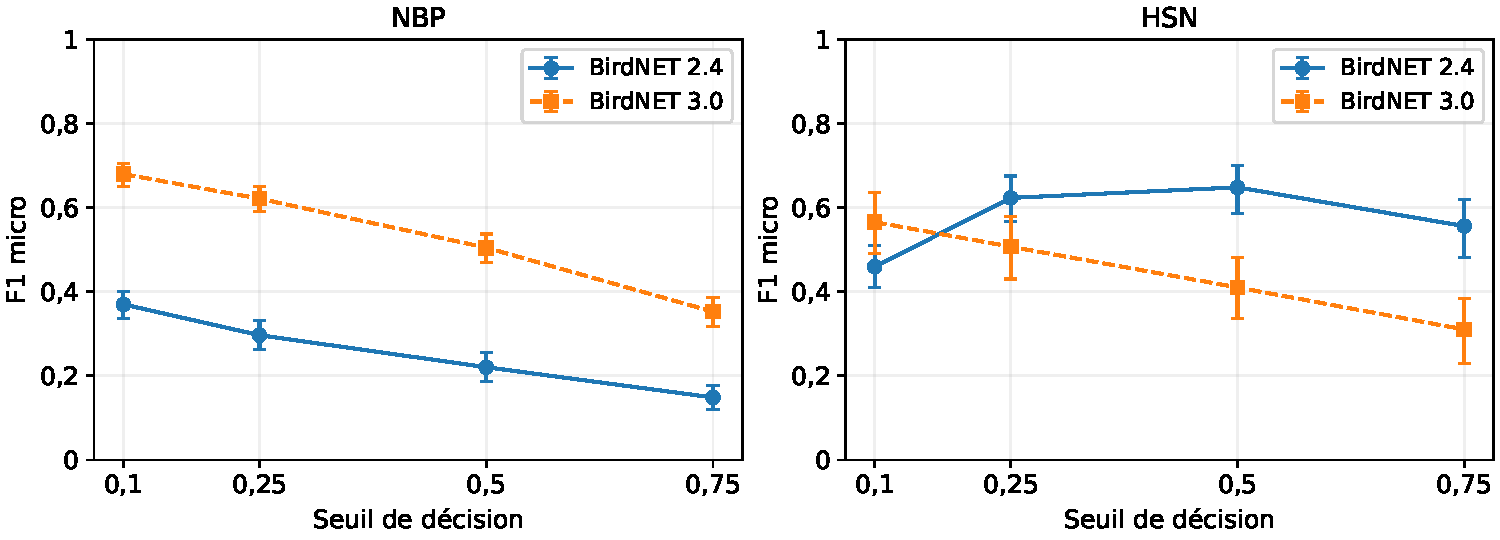
\includegraphics[width=\textwidth]{../data/results/benchmark/benchmark_f1.pdf}
\caption{F1 micro sur tous les segments aux quatre seuils communs. Les IC à
95\,\% regroupent les segments par source. Cette comparaison précède le
réglage séparé des seuils sur la partition de calibration.}
\label{fig:benchmark}
\end{figure*}

BirdNET 2.4 est exécuté en simple précision sur 32 bits (FP32) avec LiteRT,
3.0 Preview 3.1 en FP32 avec ONNX Runtime. La bibliothèque BirdNET 1.1.1
découpe les deux versions en fenêtres de trois secondes. Les mêmes extraits
sont fournis aux deux modèles, sans filtrage géographique. Le score d'une
espèce est le maximum sur les fenêtres et les sorties rattachées à son concept
taxonomique. Une espèce NBP absente de 2.4 reçoit un score nul ; les résultats
sont aussi recalculés sur les 50 classes communes. Les sorties hors du
vocabulaire annoté sont exclues : le test concerne un ensemble fermé de classes.

L'espèce absente de 2.4 est \emph{Curruca cantillans}, avec 33 présences NBP.
Elle est comptée comme omission, sans substitution par une espèce voisine.
Neuf catégories de référence correspondent à plusieurs sorties de 3.0 après
des séparations taxonomiques ; leur maximum conserve le concept annoté, avec
plusieurs possibilités de franchir le seuil. Le recalcul sur les classes
communes sert à vérifier si le changement de vocabulaire explique l'écart.

\begin{table*}[!t]
\centering\small
\caption{Évaluation sur des sources séparées de celles du réglage du seuil.
Les IC à 95\,\% rééchantillonnent les sources de test au seuil fixé.}
\label{tab:validation}
\begin{tabular}{lrrrrrr}
\toprule
\ReportDataset & \ReportVersion & \ReportThreshold & \ReportSourceSplit & \ReportPrecision & \ReportRecall & \ReportFOneNineFiveInterval \\
\midrule
NBP & 2.4 & \num{0.05} & 135 / 404 & \num{0.669} & \num{0.311} & \num{0.425} [\num{0.388}\,; \num{0.461}] \\
NBP & 3.0 & \num{0.05} & 135 / 404 & \num{0.695} & \num{0.636} & \num{0.664} [\num{0.633}\,; \num{0.694}] \\
HSN & 2.4 & \num{0.50} & 25 / 75 & \num{0.849} & \num{0.533} & \num{0.655} [\num{0.589}\,; \num{0.716}] \\
HSN & 3.0 & \num{0.05} & 25 / 75 & \num{0.741} & \num{0.508} & \num{0.603} [\num{0.533}\,; \num{0.667}] \\
\bottomrule
\end{tabular}

\end{table*}

Une partition réserve 25\,\% des sources au choix du seuil, sur une grille de
0,05 à 0,95 par pas de 0,05, en maximisant le F1 micro. Le seuil est ensuite
figé sur les autres sources ; les segments d'une même source HSN restent
groupés. La graine est \texttt{20261008}. La précision rapporte les présences
retrouvées aux prédictions retenues, le rappel aux présences annotées ; le
F1 micro réunit les décomptes des espèces. Les intervalles de confiance (IC)
à 95\,\% utilisent \num{2000} tirages bootstrap appariés par source. Ils sont
conditionnels au seuil choisi. Cette validation est interne et rétrospective ;
l'indépendance des données vis-à-vis du préentraînement n'a pas été établie.

Les seuils communs 0,10, 0,25, 0,50 et 0,75 décrivent d'abord le comportement
des modèles sur tous les segments. La validation séparée répond ensuite à la
question du réglage : 135 sources NBP et 25 sources HSN servent à choisir le
seuil ; les 404 extraits NBP et les 450 segments des 75 sources HSN restantes
servent à l'évaluation. L'appariement conserve les mêmes observations pour les
deux versions, au lieu de déduire un écart du seul chevauchement de deux IC.

\subsection{Perturbations avec contrôles acoustiques}

Les contrôles acoustiques utilisent 40 sources positives par jeu, choisies par
annotation dans le test, en conservant les omissions initiales. BirdNET 3.0
est évalué au seuil calibré de 0,05. Des bruits gaussiens ou fonds HSN enregistrés
sont ajoutés à 20, 10, 5 et 0~dB, avec cinq répétitions. À 0~dB, la puissance
du bruit ajouté égale celle de l'extrait entier, ambiance comprise. Les fonds
proviennent de 20 sources de calibration distinctes des sources positives ;
le bootstrap conserve ces groupes de fond partagé après moyenne des répétitions.
La récupération est la moyenne des proportions d'espèces annotées retrouvées
par extrait. Les mélanges réunissent 20 paires NBP et 19 paires HSN disjointes,
à ensembles d'espèces annotées disjoints, après égalisation des niveaux efficaces (RMS).
Les coefficients 50/50, 75/25 et 90/10 sont appliqués aux deux témoins isolés
et au mélange, avec un gain final commun. Le bootstrap rééchantillonne les paires.

Le SNR est réglé sur la puissance de l'extrait entier : une valeur de 0~dB
n'implique pas que le bruit ait la même puissance que le chant seul. Les ratios
de mélange désignent des coefficients d'amplitude après égalisation RMS,
pas des proportions d'espèces ou de durée. Conserver les mêmes découpages et
gains dans les témoins rend la comparaison sensible à la superposition ajoutée.
Les cinq réalisations d'un bruit ne sont pas traitées comme cinq nouvelles
sources indépendantes.

\section{Résultats retenus}

\subsection{Effet du seuil et comparaison des versions}

Dans l'exploration Xeno-canto, relever le seuil de 0,10 à 0,75 réduit
la récupération de l'espèce principale de 84,1 à 60,0\,\%. Le nombre de
prédictions par fenêtre passe de \num{98117} à \num{23583}, et les catégories
distinctes de \num{3519} à 960. Ces catégories prédites ne sont pas un
inventaire validé : les étiquettes disponibles ne décrivent pas toutes
les vocalisations présentes.

Au seuil 0,10, le F1 micro sur NBP atteint 0,679 pour 3.0 contre 0,370
pour 2.4, avec une différence appariée de $\num{+0.310}$ et un IC à 95\,\%
de $[\num{+0.277}\,;\num{+0.344}]$. Sur HSN, 2.4 obtient un rappel de
0,864 et une précision de 0,313, contre 0,434 et 0,812 pour 3.0. Parmi les
333 segments sans annotation d'oiseau, 66,4\,\% reçoivent au moins une
prédiction avec 2.4, contre 2,1\,\% avec 3.0. La version 3.0 est plus
sélective à ce seuil sur HSN, en laissant aussi davantage de présences de côté.

Après réglage séparé des seuils (tableau~\ref{tab:validation}), le F1 micro
sur NBP atteint \num{\NBPTwoFOne} pour 2.4 et \num{\NBPThreeFOne} pour 3.0.
L'écart apparié vaut \num{\NBPCalibratedDifference}, avec un IC de
$[\num{\NBPCalibratedLower}\,;\num{\NBPCalibratedUpper}]$.
Sur HSN, les F1 valent \num{\HSNTwoFOne} et \num{\HSNThreeFOne}, pour un
écart de \num{\HSNCalibratedDifference} et un IC de
$[\num{\HSNCalibratedLower}\,;\num{\HSNCalibratedUpper}]$.
L'intervalle contient zéro : aucun avantage n'est établi dans cette partition,
sans démonstration d'équivalence. Au seuil commun 0,50 sur l'ensemble HSN,
les F1 étaient de 0,648 et 0,410. Le changement de partition empêche d'attribuer
toute la réduction de l'écart au seul réglage du seuil.

La figure~\ref{fig:benchmark} explique pourquoi le seuil commun ne suffit
pas au choix d'une version. Sur NBP, 3.0 reste devant aux quatre seuils
explorés ; sur HSN, l'ordre change. Relever le seuil peut améliorer le F1
d'un modèle trop peu sélectif, puis le dégrader lorsque les omissions
deviennent trop nombreuses. Le tableau~\ref{tab:validation} présente le
compromis retenu pour chaque couple modèle/jeu sur des sources séparées.

\subsection{Bruit et vocalisations simultanées}

\begin{figure*}[!t]
\centering
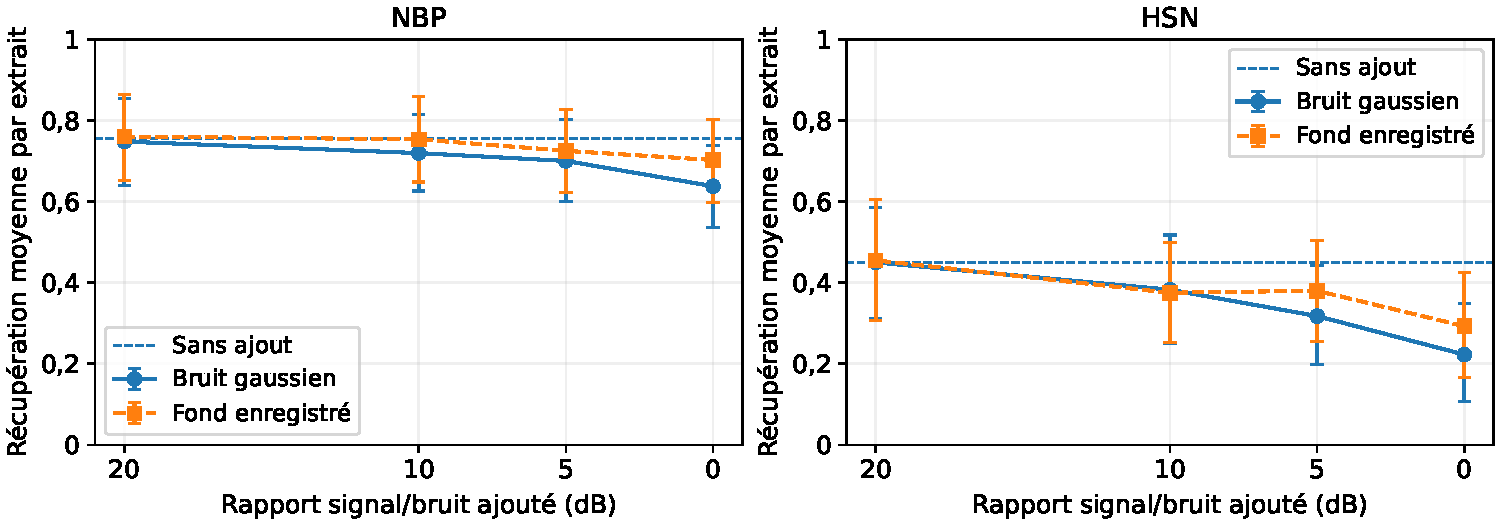
\includegraphics[width=\textwidth]{../data/results/controlled/noise/comparison.pdf}
\caption{Récupération moyenne des espèces annotées par extrait, BirdNET 3.0 au
seuil 0,05. Les tirets horizontaux indiquent les mêmes extraits sans ajout.
Les barres sont des IC à 95\,\%, groupés par source de fond partagé.}
\label{fig:noise}
\end{figure*}

Sans perturbation, la récupération moyenne par extrait est de
\num{\NBPControlledClean}\,\% sur NBP et \num{\HSNControlledClean}\,\% sur HSN.
À 0~dB, elle atteint respectivement \num{\NBPGaussianZero}\,\% et
\num{\HSNGaussianZero}\,\% avec le bruit gaussien, puis
\num{\NBPNaturalZero}\,\% et \num{\HSNNaturalZero}\,\% avec les fonds
enregistrés (figure~\ref{fig:noise}). Les quatre IC appariés de l'écart avec
l'original sont entièrement négatifs. L'exploration Xeno-canto retrouvait
82,5\,\% des cibles à 0~dB contre 99,9\,\% sur les segments originaux,
mais sous condition de reconnaissance préalable. Les valeurs absolues ne
décrivent donc pas une même sensibilité.

Dans l'exploration, le score moyen exporté passe de 0,778 à 0,568 à 0~dB.
L'écart apparié vaut $\num{-0.211}$, avec un IC à 95\,\% de
$[\num{-0.219}\,;\num{-0.203}]$ ; le regroupement par espèce l'élargit à
$[\num{-0.252}\,;\num{-0.181}]$. Le signe de la baisse est conservé dans
les deux calculs. Ces scores exportés sont censurés sous le seuil 0,10,
où ils sont représentés par zéro : leur moyenne décrit les sorties retenues,
pas toute la réponse interne du réseau.

\begin{table*}[!t]
\centering\small
\caption{Récupération conjointe à 50/50 dans les témoins isolés et le mélange,
sur 20 paires NBP et 19 paires HSN. L'écart mélange moins témoins est en points
de pourcentage ; les IC à 95\,\% rééchantillonnent les paires disjointes.}
\label{tab:overlap}
\begin{tabular}{lrrr}
\toprule
Jeu & Témoins isolés & Mélange & Écart (points) [IC 95\,\%] \\
\midrule
NBP & \num{\NBPIsolatedBoth}\,\% & \num{\NBPMixedBoth}\,\% & \num{-30.0} [\num{-50.0}\,; \num{-10.0}] \\
HSN & \num{\HSNIsolatedBoth}\,\% & \num{\HSNMixedBoth}\,\% & \num{-21.1} [\num{-42.1}\,; \num{-5.3}] \\
\bottomrule
\end{tabular}
\end{table*}

La récupération des deux cibles baisse aussi lors des mélanges par rapport
aux témoins isolés (tableau~\ref{tab:overlap}). Sur NBP, elle passe de 30,0
à 20,0 puis 10,0\,\% entre 50/50, 75/25 et 90/10, contre 60,0\,\% dans les
témoins à chaque ratio. Sur HSN, une seule paire sur 19 retrouve les deux
cibles dans chaque mélange ; à 90/10, l'IC de l'écart atteint zéro.
Ce résultat identique sur trois ratios ne démontre pas une insensibilité
au niveau relatif, compte tenu des effectifs et des intervalles larges.

Dans les \OverlapPairs{} paires exploratoires Xeno-canto, la récupération
conjointe vaut 26,8\,\% à 50/50, avec un IC à 95\,\% de
$[\num{24.4}\,;\num{29.0}]$\,\%, contre 18,6\,\% à 90/10. Ces mélanges
sans égalisation ne séparent pas l'effet du ratio de celui des niveaux
initiaux. Les essais BirdSet avec témoins isolés apportent cette comparaison
contrôlée sur un effectif plus réduit.

\section{Interprétation et discussion critique}

\subsection{Ce que les perturbations apprennent sur la robustesse}

Le biais de sélection explique une partie de l'écart entre les deux volets.
L'exploration Xeno-canto retient les cibles déjà reconnues et leur meilleur
segment, alors que les contrôles BirdSet gardent les omissions initiales.
J'en retiens qu'un taux élevé sous bruit n'est interprétable qu'en connaissant
son dénominateur et sa sélection. La baisse à 0~dB persiste sur les extraits
choisis par annotation : elle ne dépend donc pas uniquement du premier biais.
Les deux expériences confortent ce constat dans leurs conditions, sans
autoriser la mise en commun de leurs taux.

La même attention à l'agrégation vaut pour le corpus initial : à 0~dB,
la récupération vaut 82,5\,\% en donnant le même poids aux enregistrements,
contre 78,0\,\% en donnant le même poids aux espèces. L'écart est cohérent
avec la forte concentration des données. Ajouter des exemples d'une espèce
déjà dominante augmente la précision de sa description, mais renseigne peu
les espèces rares du corpus.

Les fonds enregistrés donnent des récupérations moyennes plus élevées que le
bruit gaussien à 0~dB, à puissance ajoutée contrôlée. Une explication possible
est leur répartition spectrale et temporelle différente ; elle n'a pas été
mesurée. Les IC calculés portent sur l'écart à l'original, sans test apparié
direct entre types de bruit. Les fonds ne sont ni caractérisés comme pluie,
vent ou insectes, ni certifiés exempts de toute vocalisation. Un SNR identique
ne suffit donc pas à qualifier une difficulté acoustique identique.

Les témoins isolés distinguent les omissions présentes avant mélange de la
difficulté ajoutée par la superposition. L'écart négatif à 50/50 est compatible
avec un effet de masquage supplémentaire, mais le découpage et l'égalisation
portent sur les extraits entiers, sans séparer les chants de leurs ambiances.
Les augmentations par mélanges de Perch 2.0 et Bird-MAE répondent à ce problème
pendant l'apprentissage\cite{perch2025,birdmae2025}. Elles constituent un point
de comparaison pertinent, dont l'efficacité relative n'est pas mesurée ici.

\subsection{Choisir un modèle et un seuil pour un usage donné}

L'avantage de 3.0 sur NBP persiste après réglage du seuil. À seuil commun 0,10,
la restriction aux 50 classes partagées donnait également des F1 de 0,678
pour 3.0 et 0,380 pour 2.4 : l'écart ne se réduit pas à l'espèce absente de 2.4.
HSN montre une autre situation, où l'écart dépend davantage de la décision.
Cela rejoint les compromis décrits par Pérez-Granados\cite{perez2023}.
Pour une migration de version, je conserverais les données de validation,
réviserais le seuil et vérifierais les correspondances taxonomiques, plutôt
que de transposer un réglage numérique à l'identique.

La calibration désigne ici le choix d'un seuil, pas une transformation des
scores en probabilités calibrées. Trois des quatre couples modèle/jeu
retiennent 0,05, borne inférieure explorée ; le meilleur seuil de la grille
n'est pas nécessairement optimal sur tout l'intervalle des scores. Le F1 micro
privilégie les présences fréquentes : sur les 11 espèces HSN présentes dans le
test, le F1 macro vaut 0,509 pour 2.4 et 0,560 pour 3.0, contrairement à
l'ordre micro. Une recherche centrée sur une espèce rare peut donc demander
un autre réglage. Une partition unique et des IC conditionnels au seuil ne
mesurent pas la variabilité de toute la procédure de sélection.

Le choix technologique dépasse cette comparaison locale. Pour analyser des
archives dans un vocabulaire couvert, BirdNET fournit une chaîne directement
utilisable ; 3.0 reste néanmoins une préversion dont les conditions de
distribution demandent clarification. Pour de nouvelles classes ou des types
de cris, un classifieur sur représentations gelées offre un premier essai
avant l'ajustement complet, cohérent avec les travaux de transfert
\cite{ghani2023,ghani2025}. AVES et Bird-MAE apportent d'autres représentations
à comparer avec les mêmes annotations et le même protocole. La maturité des
outils, les licences et le coût d'extraction doivent être examinés séparément
des performances annoncées dans des évaluations différentes.

\subsection{Portée de l'étude et verrous qui subsistent}

Le test se limite aux catégories annotées ; les alertes hors vocabulaire
ne sont pas comptabilisées. Les correspondances taxonomiques sont en partie
asymétriques, et l'usage d'un maximum sur plusieurs sorties pour certains
concepts de 3.0 ne rend pas les vocabulaires strictement identiques.
Les 40 extraits par jeu et les 20 sources de fond restreignent aussi la
précision des contrôles acoustiques. Les intervalles décrivent le corpus
observé, sans corriger toutes les dépendances entre sites ou auteurs.

NBP et HSN ne partagent aucune espèce dans leurs vocabulaires évalués ; les
métadonnées disponibles ne permettent pas une comparaison multisite
contrôlée. L'écart entre jeux combine donc des effets taxonomiques, acoustiques
et géographiques. L'étude ne tranche pas la question du transfert vers une
nouvelle région, ni celle d'un éventuel recouvrement avec le préentraînement.
Les évaluations de Sethi et de Funosas montrent l'intérêt d'une validation
locale et de plusieurs sites\cite{sethi2024,funosas2026}, que cette
expérimentation réduite ne remplace pas.

\section{Conclusion et prise de recul}

Les modèles permettent d'automatiser une partie de l'identification des oiseaux,
mais le bruit, les superpositions et les données de référence conditionnent
la portée de leurs sorties. Les expériences établissent une dégradation dans
les perturbations étudiées ; elles ne classent pas toutes les technologies.
BirdNET 3.0 présente un avantage sur NBP ; sur HSN, le choix dépend du seuil
et du critère. La généralisation géographique demeure
non résolue par les données utilisées.

Je retiens qu'il faut évaluer ensemble modèle, annotations et décision.
Pour un usage direct, je partirais d'un modèle distribué et d'un ensemble
local annoté ; pour des catégories absentes, d'une adaptation de
représentations. La priorité serait un test multisite sur des espèces
communes, avec des sites ou campagnes réservés dès le départ à l'évaluation.
Modèles directs et adaptations seraient comparés avec le même budget
d'annotations. Pour Bird-MAE, j'inclurais une tête à prototypes en plus
d'une tête linéaire.

Les contrôles acoustiques gagneraient à utiliser des fonds caractérisés et
davantage de paires réannotées après découpage. Le débit, la mémoire et la
stabilité restent à mesurer sur le matériel visé. Accumuler uniquement des
sons focaux ne résoudrait ni le biais de sélection, ni les erreurs d'un
inventaire ouvert.

% Start references on a separate page so the six-page limit is unambiguous.
\FloatBarrier
\label{report:body-end}
\clearpage
\bibliographystyle{unsrt}
\bibliography{references}

\end{document}
